\chapter{\texorpdfstring{\acrshort{knn}}{kNN} queries in the snapshot model}\label{section:knn-snapshot}
\thispagestyle{myheadings}

	In this chapter I analyze secure \acrshort{knn} queries in the snapshot adversary model.
	I study the effect of protecting the records with a type of property-preserving encryption on quality of search and efficiency of certain attacks.
	Specifically, I examine theoretically and practically how accuracy of both \acrshort{knn} search and \acrshort{ml}-based inversion attack degrade with added security.

	\section{Introduction}

		Nearest-neighbor search is a type of optimization problem that, given a set of objects and a distance metric, requires finding the object closest to a given object according to the distance metric.
		A \acrfull{knn} search is a subtype of a general nearest-neighbor problem where $k$ closest objects are requested.
		Applications that use \acrshort{knn} search only need to define the objects and the metric.
		For example, a street map application would define the 2D coordinates of the buildings as objects and Euclidean distance as a metric, then the query could be ``give 5 restaurants closest to the current user position''.
		A document search application would define the keyword vector for a document as an object and an inner product distance as a metric, then the query could be ``give 3 documents most similar to the given text'' (similar applications may search images, videos and sounds).

		In this chapter we propose a method and an analysis of running secure \acrshort{knn} queries in outsourced database model.
		We model our application as a generic document similarity search, where the server stores the embeddings of the documents and returns $k$ closest records to the query embedding.
		We propose to apply a type of property-preserving encryption over the embeddings on the server while retaining its ability to do nearest-neighbor search.
		Finally, we simulate an attack against the records --- an \acrshort{ml}-based inversion attack that aims to recover the set of words of a document from its embeddings.
		Our goal is to observe and study the correlation of the security parameter with search accuracy and attack efficiency.

		To summarize, our contributions in this work are as follows:
		\begin{itemize}
			\item
				We adapt and implement a \acrfull{dcpe} scheme from \cite{dcpe} to encrypt text embeddings.
				We analyze the practical aspects of \acrshort{dcpe} scheme's security (e.g., the effects of floating point representation) and benchmark the construction.

			\item
				We conduct a set of experiments to study the effect of security parameter on search accuracy.
				We use a fine-tuned \acrshort{bert} model\footnote{Provided by Hamed Zamani} to produce embeddings for the \acrshort{trec} 2020 collection.
				Given \acrshort{trec} validation set (i.e., ``correct answers'') we run the search for varying security levels and report a number of ranking quality measures.

			\item
				We adapt a recent \acrshort{ml}-based inversion attack by \textcite{embedding-attacks} against embeddings to our setting.
				The attack works by training an \acrshort{lstm} model on pairs of sentences and their embeddings.
				We run this attack for varying security levels, and training on both plaintext and encrypted records.

			\item
				Finally, we analyze the correlation results for search accuracy and attack efficiency and conclude on practicality of our method.
		\end{itemize}

	\section{Related Work}

		Work in this area is naturally split into two groups --- mechanisms and constructions that offer certain security guarantees for nearest-neighbor queries, and attacks against those constructions.

		A work immediately related to ours is that of \textcite{quick-n}.
		QuickN offers an adaptation of nearest-neighbor search algorithm in conventional tree data structures (i.e., R-trees) to well-established \acrfull{ope} schemes.
		Unlike our solution that involves a novel property-preserving encryption scheme specifically designed for high-dimensional vectors, QuickN encrypts each vector dimension separately with \acrshort{ope}.
		\cite{quick-n} includes the experiments with attacks against their solution (attack of \textcite{leakage-abuse-grubs-2017}) and report high degree of protection against them.

		QuickN approach of applying \acrshort{ope} to an R-tree, however, has some disadvantages.
		First, an ideal stateless \acrshort{ope} has been shown inferior (\cite{ope-leakage}) to its counterpart, an \acrfull{ore} in which the comparison over ciphertexts is defined explicitly.\footnote{
			\cite{quick-n} uses mOPE \cite{ope-ideal-security-protocol} which is an interactive protocol and not a traditional lightweight stateless \acrshort{ope} like \cite{bclo-ope}.
			Since mOPE is an ideal (though stateful) \acrshort{ope}, \cite{quick-n} do not include \acrshort{ope} leakage in their security definition.
		}
		An \acrshort{ore}, in turn, can have a varying level of security, with the higher security level translating into lower comparison performance.
		In QuickN, an R-tree-based nearest-neighbor algorithm involves a very high number of comparisons, linear in data dimensionality.
		With the cost of comparison no longer negligible, the overhead of query over 2D or 3D is already high, saying nothing of 768-dimensional vectors that our work targets.
		Second, QuickN protocol is not single-round (i.e., it takes two roundtrips per query) and it returns a large number of false positive results even for a minimal $k$ (\num{4000} false positives for $10^6$ dataset and $k = 1$).

		\textcite{knn-aspe} offer a novel scheme, ASPE, that preserves a special type of scalar product.
		ASPE is then naturally integrated in existing \acrshort{knn} algorithms that rely on a scalar product.
		\cite{knn-aspe} is similar to ours in that we also apply a property-preserving encryption scheme to existing \acrshort{knn} algorithms.
		ASPE is different in that it preserves a scalar product while we preserve an L2 distance comparison, and ASPE has been broken in \cite{secure-nn-revisited-break-aspe} (although an attack is a chosen plaintext attack, i.e., one cannot decrypt a random ciphertext).

		Other works either target different aspects of query security, like integrity and soundness of results \cite{knn-integrity-soundness,svknn}, or involve mechanisms other than property-preserving encryption \cite{seceqp,practical-approx-knn,knn-sharing-keys,knn-mult-data-owners,knn-over-encrypted,knn-paillier,knn-blind,knn-homomorphism,knn-strong-location-privacy,knn-no-anonymizers,knn-efficient,knn-new-casper}.

	\section{\texorpdfstring{\acrlong{dcpe}}{Distance Comparison Preserving Encryption}}

		A promising approach in secure \acrshort{knn} evaluation is using a property-preserving encryption scheme to allow the existing search algorithms to work with minimal alterations.
		ASPE scheme by \textcite{knn-aspe} is a step in this direction, but a scheme has been shown insecure under a type of chosen plaintext attack in \cite{secure-nn-revisited-break-aspe}.
		Using a common \acrshort{ope} scheme over vector values has been explored in \cite{quick-n}, but this approach incurs high overhead linear in dimensionality.
		We, therefore, need a different method --- a scheme that operates over high-dimensional vectors and preserves a property that is required to answer the nearest-neighbor queries.

		A classical nearest-neighbor search \cite{knn-wong,knn-cunningham} simply orders the objects according to their distances from the target.
		It is important to note that knowing the exact distance is not required, merely the knowledge of \emph{distance comparison} suffices (i.e., $x$ is closer to $y$ than $z$ is).
		An encryption scheme that preserves the distance comparison would satisfy the \acrshort{knn} search correctness, but not necessarily security or even practicality.
		First, a fully deterministic \acrfull{dcpe} would reveal at least the frequency of data points (i.e., how many times a point appears in the dataset).
		Second, even in the plaintext world the use of approximate nearest-neighbor search \cite{scalable-nn,approximate-nn-fixed-d} may be preferred due to the curse of dimensionality \cite{nn-meaningful,nn-curse-of-d} (exact distance is less important in higher dimensions).

		A candidate \emph{approximate} \acrshort{dcpe} scheme that we adapt to our solution has been recently proposed by \textcite{dcpe}.
		The scheme provides the following guarantee on its ciphertexts
		\begin{multline*}
			\forall x, y, z \in \mathbb{X} : \algo{Dist}{x, y} < \algo{Dist}{x, z} - \beta \\
			\implies \algo{Dist}{f(x), f(y)} < \algo{Dist}{f(x), f(z)}
		\end{multline*}
		where $\mathbb{X} \subseteq \mathbb{R}^d$ is the set of $d$-dimensional vectors of real numbers, \algo{Dist} is the inner product distance over elements in $\mathbb{X}$, and $\beta$ is the approximation term.
		Parameter $\beta$ partially defines the security of the encrypted set --- the larger $\beta$, the fewer distance comparisons are preserved, the less accurate the search and the reconstruction attacks would be.
		\textcite{dcpe} prove protection against membership inference attacks \cite{memebership-inference-attacks-knn} (whether an individual is in the database or not), and against approximate frequency-finding attacks (how many times the element appears in the set, see \cite{leakage-abuse-grubs-2017} for \acrshort{ore} frequency attacks).
		As for the choice of $\beta$, \textcite{dcpe} proves that $\beta \approx \sqrt{\max N}$ would hide about half of the input bits, for $\max N$ being the maximum vector length in the dataset.

		% chktex-file 1
% chktex-file 8

\newlength{\dcpeAlgInterLength}
\setlength{\dcpeAlgInterLength}{0.18ex}

\begin{algorithm*}[ht!]

	\begin{pchstack}

		\procedure[linenumbering]{\algo{KeyGen}{\secparam, \mathbb{S}}}{
			s \sample \mathbb{S}		\\
			\key \sample \bin^\secpar	\\
			\pcreturn (s, \key)
		}

		\hspace{\dcpeAlgInterLength}

		\procedure[linenumbering]{\algo{Enc}{ (s, \key), \vec{m} }}{
			n \sample \bin^\secpar														\\
			\mathsf{coins}_n || \mathsf{coins}_u \gets \algo{\acrshort{prf}}{\key, n}	\\
			\vec{n} \sample \algo{Normal}{0, I_d; \mathsf{coins}_n}						\\
			u \sample \algo{Uniform}{0, 1; \mathsf{coins}_u}							\\
			x \gets \frac{s \beta}{4} \cdot \sqrt[d]{u}									\\
			\vec{\delta} \gets \frac{\vec{n}}{\|\vec{n}\|} \cdot x						\\
			\vec{c} \gets s \cdot \vec{m} + \vec{\delta}								\\
			\pcreturn \vec{c}
		}

		\hspace{\dcpeAlgInterLength}

		\procedure[linenumbering]{\algo{Dec}{ (s, \key), (\vec{c}, n) }}{
			\mathsf{coins}_n || \mathsf{coins}_u \gets \algo{\acrshort{prf}}{\key, n}	\\
			\vec{n} \sample \algo{Normal}{0, I_d; \mathsf{coins}_n}						\\
			u \sample \algo{Uniform}{0, 1; \mathsf{coins}_u}							\\
			x \gets \frac{s \beta}{4} \cdot \sqrt[d]{u}									\\
			\vec{\delta} \gets \frac{\vec{n}}{\|\vec{n}\|} \cdot x						\\
			\vec{m} \gets \frac{\vec{c} - \vec{\delta}}{s}								\\
			\pcreturn \vec{m}
		}

	\end{pchstack}

	\caption[\acrshort{dcpe} scheme]{
		\acrlong{dcpe} scheme, adapted from \cite[Algorithm 2]{dcpe}.
	}%
	\label{algorithm:dcpe}
\end{algorithm*}


		\textcite{dcpe} offer an instantiation of the $\beta$-\acrshort{dcpe} scheme (though not an implementation) that we have adapted for our needs and show on \cref{algorithm:dcpe}.

		The \algo{KeyGen} procedure generates a key \key{} and an amplification factor $s$.

		The \algo{Enc} procedure ``encrypts'' an object by moving it in space in a way that it is hard to recover its original position and its distance-comparison respective to other encrypted points is preserved.
		The algorithm first constructs a hyperball of radius $\beta$, the approximation term, around the input point.
		The routine then samples a new point uniformly inside that hyperball.
		Finally, that new point is projected into the ciphertext point according to the amplification factor $s$.
		Note that for each encryption the scheme generates a nonce $n$ and uses it along with the key \key{} to generate the coins for the samplers.
		That is, the point in the $\beta$-hyperball is deterministically set from the nonce (unique per point) and the key (one for all points), and the final ciphertext is scaled the same way for all points.
		The \algo{Dec} procedure makes the same steps in reverse correctly setting the point in the hyperball using the nonce and the key.

		\begin{figure}[!ht]
	\centering
	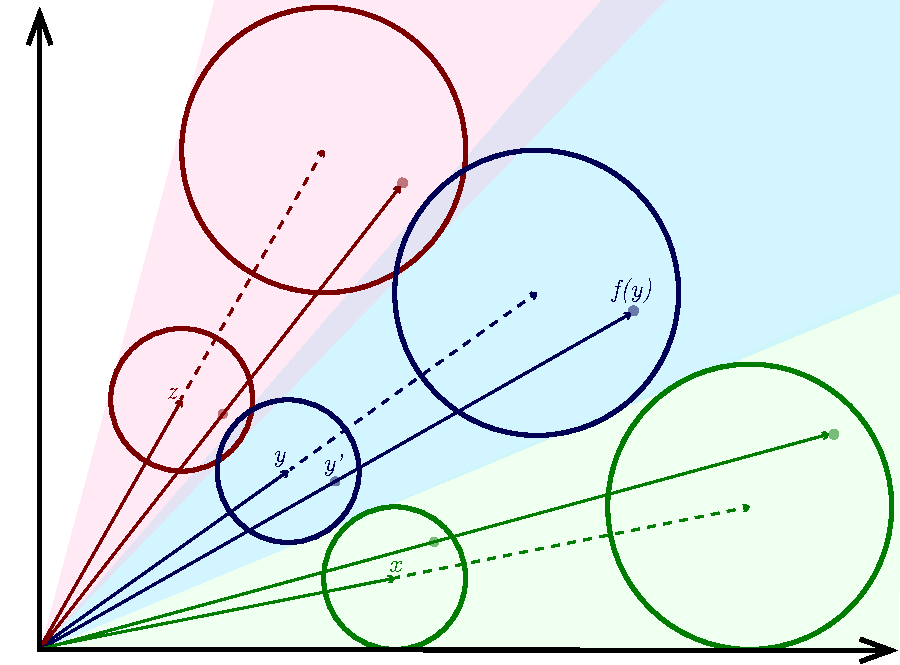
\includegraphics[width=1.0\textwidth]{dcpe}
	\caption[Schematic description of \acrshort{dcpe}]{
		Schematic description of encryption process of \acrshort{dcpe}, drawn to scale.
		In this diagram, there are two dimensions ($d = 2$), $\beta$ (the radius of a circle) is 2 units, and $s$ (the projection magnitude, the length from the origin to the larger circle over the length to the smaller one) is 2.
		The encrypted point is uniformly sampled inside a $\beta$-sphere, then projected $s$ times further from the origin.
		If two points are too close, their circles intersect, and their encryptions can be sampled in a way that breaks distance comparison.
		Intuitively, larger $\beta$ implies greater ciphertext space for a point and greater security.
	}\label{figure:dcpe}
\end{figure}


		The security of the scheme thus depends on
		\begin{enumerate*}[label={(\roman*)}]
			\item the maximum amount of amplification,
			\item the radius of the hyperball $\beta$, and
			\item the entropy of the samplers.
		\end{enumerate*}
		\textcite{dcpe} show that the amplification, $s$ parameter, affects one-wayness bounds \cite[Section 7.2]{dcpe}.
		Approximation term $\beta$ affects bit-security with $\beta \approx \sqrt{\max N}$ protecting about half of the bits.
		Finally, the key \key{} and nonce $n$ sizes, the security parameter \secparam{}, and the samplers used to generate normal multivariate and uniform samples affect the specific amount of entropy used to generate a point in the hyperball.

		As the construction operates on real numbers, an open question remains on how to avoid negative side-effects of floating point numbers bit representation.
		Unlike integers, floating point numbers are represented in memory in a way that their precision is different depending on their value, see the IEEE 754-2019 standard \cite{ieee-floating-point}. % chktex 8
		Simply put, the closer the value is to zero, the smaller the difference between two consecutive representable values is.
		For example, while the representable 32-bit IEEE 754 floating point numbers range from about $1.18 \cdot 10^{-38}$ to $3.4 \cdot 10^{38}$, there are only $2^{32} \approx 4 \cdot 10^9$, 4 billion representable numbers.
		This, along with the rounding errors, puts some limits on how large $s$ and $\beta$ can be.

		We offer the first implementation of \cite{dcpe} $\beta$-\acrshort{dcpe} for 32- and 64-bit IEEE 754 numbers in C++.\footnote{
			\url{https://github.com/private-knn/dcpe}
		}
		The code is documented, tested and benchmarked, see \cref{table:dcpe-benchamrks}.
		Observe that the difference in performance between encryption and decryption is predictably minimal, and the overhead of encryption grows slower than linearly with dimensionality.
.
		{
	\def\arraystretch{1.0}
	\begin{table}[!ht]
		\begin{tabular*}{\linewidth}{ !{\extracolsep\fill} l l c l } % chktex 26
			\toprule
				Operation						& Input size								& Dimensions $d$	& Wall-clock time			\\
			\midrule
				\algo{KeyGen}					& N/A										& N/A				& \SI{1.81}{\milli\second}	\\
			\midrule
				\multirow{6}{*}{\algo{Enc}}		& \multirow{3}{*}{32-bit (\texttt{float})}	& 1					& \SI{4.12}{\milli\second}	\\
												& 											& 100				& \SI{12.2}{\milli\second}	\\
												& 											& 768				& \SI{62.0}{\milli\second}	\\ \cline{2-4}
												& \multirow{3}{*}{64-bit (\texttt{double})}	& 1					& \SI{3.96}{\milli\second}	\\
												& 											& 100				& \SI{11.4}{\milli\second}	\\
												& 											& 768				& \SI{59.3}{\milli\second}	\\
			\midrule
				\multirow{6}{*}{\algo{Dec}}		& \multirow{3}{*}{32-bit (\texttt{float})}	& 1					& \SI{3.94}{\milli\second}	\\
												& 											& 100				& \SI{11.6}{\milli\second}	\\
												& 											& 768				& \SI{62.1}{\milli\second}	\\ \cline{2-4}
												& \multirow{3}{*}{64-bit (\texttt{double})}	& 1					& \SI{3.96}{\milli\second}	\\
												& 											& 100				& \SI{11.3}{\milli\second}	\\
												& 											& 768				& \SI{59.6}{\milli\second}	\\
			\bottomrule
		\end{tabular*}
		\caption{\acrshort{dcpe} implementation benchmarks}%
		\label{table:dcpe-benchmarks}
	\end{table}
}

% cSpell:disable

% ref: e9fd950
% ❯ make clean run-benchmarks                                                                             04:24:23 PM
% rm -rf ../docs
% rm -rf bin/*
% rm -rf obj/* *~ *.dSYM *.gcov *.gcda *.gcno *.bin coverage-html junit-*.xml cobertura.xml
% clang++ -c -o obj/utility.o src/utility.cpp -I/opt/homebrew/opt/openssl@3/include -I/opt/homebrew/Cellar/boost/1.76.0/include -I/opt/homebrew/opt/llvm/include --std=c++2a -Wall -Wno-unknown-pragmas -fPIC -I include
% clang++ -c -o obj/scheme.o src/scheme.cpp -I/opt/homebrew/opt/openssl@3/include -I/opt/homebrew/Cellar/boost/1.76.0/include -I/opt/homebrew/opt/llvm/include --std=c++2a -Wall -Wno-unknown-pragmas -fPIC -I include
% clang++ -o bin/benchmark-utility obj/utility.o obj/scheme.o benchmark/benchmark-utility.cpp -I/opt/homebrew/opt/openssl@3/include -I/opt/homebrew/Cellar/boost/1.76.0/include -I/opt/homebrew/opt/llvm/include --std=c++2a -Wall -Wno-unknown-pragmas -fPIC -I include -l boost_system  -l gtest -l pthread -l benchmark  -L/opt/homebrew/opt/openssl@3/lib -L/opt/homebrew/Cellar/boost/1.76.0/lib -L/opt/homebrew/opt/llvm/lib -L lib
% clang++ -o bin/benchmark-scheme obj/utility.o obj/scheme.o benchmark/benchmark-scheme.cpp -I/opt/homebrew/opt/openssl@3/include -I/opt/homebrew/Cellar/boost/1.76.0/include -I/opt/homebrew/opt/llvm/include --std=c++2a -Wall -Wno-unknown-pragmas -fPIC -I include -l boost_system  -l gtest -l pthread -l benchmark  -L/opt/homebrew/opt/openssl@3/lib -L/opt/homebrew/Cellar/boost/1.76.0/lib -L/opt/homebrew/opt/llvm/lib -L lib
% bin/benchmark-utility&& bin/benchmark-scheme&& echo Benchmarks completed!
% Unable to determine clock rate from sysctl: hw.cpufrequency: No such file or directory
% 2022-03-23T16:25:25-04:00
% Running bin/benchmark-utility
% Run on (10 X 24.1209 MHz CPU s)
% CPU Caches:
%   L1 Data 64 KiB (x10)
%   L1 Instruction 128 KiB (x10)
%   L2 Unified 4096 KiB (x5)
% Load Average: 3.31, 2.42, 2.17
% ------------------------------------------------------------------------------------------------------
% Benchmark                                                            Time             CPU   Iterations
% ------------------------------------------------------------------------------------------------------
% UtilityBenchmark<float>/Random/iterations:1048576                0.031 us        0.030 us      1048576
% UtilityBenchmark<float>/Uniform_float/iterations:1048576          1.68 us         1.68 us      1048576
% UtilityBenchmark<double>/Uniform_double/iterations:1048576        1.72 us         1.72 us      1048576
% UtilityBenchmark<float>/Normal_float/1/iterations:32768           1.99 us         1.98 us        32768
% UtilityBenchmark<float>/Normal_float/2/iterations:32768           2.07 us         2.07 us        32768
% UtilityBenchmark<float>/Normal_float/3/iterations:32768           2.14 us         2.14 us        32768
% UtilityBenchmark<float>/Normal_float/10/iterations:32768          2.61 us         2.61 us        32768
% UtilityBenchmark<float>/Normal_float/100/iterations:32768         7.32 us         7.32 us        32768
% UtilityBenchmark<double>/Normal_double/1/iterations:32768         1.97 us         1.97 us        32768
% UtilityBenchmark<double>/Normal_double/2/iterations:32768         2.06 us         2.06 us        32768
% UtilityBenchmark<double>/Normal_double/3/iterations:32768         2.13 us         2.13 us        32768
% UtilityBenchmark<double>/Normal_double/10/iterations:32768        2.55 us         2.55 us        32768
% UtilityBenchmark<double>/Normal_double/100/iterations:32768       7.06 us         7.06 us        32768
% Unable to determine clock rate from sysctl: hw.cpufrequency: No such file or directory
% 2022-03-23T16:25:30-04:00
% Running bin/benchmark-scheme
% Run on (10 X 24.1206 MHz CPU s)
% CPU Caches:
%   L1 Data 64 KiB (x10)
%   L1 Instruction 128 KiB (x10)
%   L2 Unified 4096 KiB (x5)
% Load Average: 3.61, 2.49, 2.20
% ------------------------------------------------------------------------------------------------------
% Benchmark                                                            Time             CPU   Iterations
% ------------------------------------------------------------------------------------------------------
% SchemeBenchmark<float>/KeyGen_float/iterations:1048576            1.81 us         1.81 us      1048576
% SchemeBenchmark<double>/KeyGen_double/iterations:1048576          1.79 us         1.79 us      1048576
% SchemeBenchmark<float>/Encrypt_float/1/iterations:32768           4.12 us         4.12 us        32768
% SchemeBenchmark<float>/Encrypt_float/100/iterations:32768         12.2 us         12.2 us        32768
% SchemeBenchmark<float>/Encrypt_float/768/iterations:32768         62.0 us         62.0 us        32768
% SchemeBenchmark<double>/Encrypt_double/1/iterations:32768         3.96 us         3.96 us        32768
% SchemeBenchmark<double>/Encrypt_double/100/iterations:32768       11.4 us         11.4 us        32768
% SchemeBenchmark<double>/Encrypt_double/768/iterations:32768       59.3 us         59.3 us        32768
% SchemeBenchmark<float>/Decrypt_float/1/iterations:32768           3.94 us         3.94 us        32768
% SchemeBenchmark<float>/Decrypt_float/100/iterations:32768         11.6 us         11.6 us        32768
% SchemeBenchmark<float>/Decrypt_float/768/iterations:32768         62.1 us         62.1 us        32768
% SchemeBenchmark<double>/Decrypt_double/1/iterations:32768         3.96 us         3.96 us        32768
% SchemeBenchmark<double>/Decrypt_double/100/iterations:32768       11.3 us         11.3 us        32768
% SchemeBenchmark<double>/Decrypt_double/768/iterations:32768       59.6 us         59.6 us        32768
% Benchmarks completed!


	\section{\texorpdfstring{\acrshort{knn}}{kNN} search accuracy}

		The first part of a practical and secure outsourced similarity search application is the search accuracy.
		In this set of experiments we embed the documents and apply $\beta$-\acrshort{dcpe} to the embeddings.
		We use existing efficient nearest-neighbor search algorithms and report on ranking quality metrics for different $\beta$.

		With the $\beta$-\acrshort{dcpe} as a component, we can model the protocols similar to \acrshort{ore} ones.
		In the setup protocol \protocolSetup{}, \user{} simply encrypts the entire input, one vector at a time, and sends the encrypted data over to \server{}.
		In the query protocol \protocolQuery{}, \user{} encrypts the query with \acrshort{dcpe}, sends the ciphertext to \server{}, while \server{} runs a standard \acrshort{knn} search against the ciphertext.
		$k$ encrypted vectors are then returned to \user{}, who decrypts them as the last step.
		These protocols are run for a single set of secrets and \acrshort{dcpe} parameters, including $\beta$.

		For the choice of the dataset, we use the established information retrieval \acrshort{trec} 2020 test collections.
		A \acrshort{trec} collection consists of a set of documents, a set of topics (questions) and a corresponding set of relevance judgments (correct answers).
		A benefit of using a \acrshort{trec} dataset is being able to evaluate relevant metrics over the produced results, for example, \acrshort{mrr} \cite{mrr} and \acrshort{dcg} \cite{dcg}.
		We can then track how these metrics, along with the simpler edit distance and set difference over the result, degrade with higher security.

		As the embedding mechanism, we use a custom fine-tuned \acrshort{bert} model.\footnote{Provided by Hamed Zamani}
		\acrfull{bert} is a transformer-based \acrshort{ml} technique for \acrlong{nlp}.
		An original \acrshort{bert} model, published by \textcite{bert}, has been trained on a BookCorpus \cite{bookcorpus} (800 million words) and English Wikipedia (2.5 billion words) using 24 encoders with 16 bidirectional self-attention heads (for the larger of two versions, $\text{\acrshort{bert}}_\text{LARGE}$).
		\acrshort{bert}'s main novelty is its bidirectional nature --- it processes all words in relation to each other and not one-by-one.
		The technology is now prevalent \cite{bert-is-prevalent}, and Google uses \acrshort{bert} in almost every English query\footnote{
			\url{https://searchengineland.com/google-bert-used-on-almost-every-english-query-342193}
		}.
		It is common, however, to use the original \acrshort{bert} model as a base and do training on top.
		{\color{red}We use one of such fine-tuned \acrshort{bert} models for embedding.}

		The actual experiment is conducted as follows.
		First, we produce a set of embeddings for 8.8 million documents and 200 queries from \acrshort{trec} 2020 dataset.
		We observed that the maximum length of an embedding vector is about 11 units.
		Second, we encrypt the data and queries embeddings using \acrshort{dcpe} and ranging $\beta$ from 0 (meaning exact distance-comparison) to 50, with $\beta = \sqrt{11} \approx 3.3$ hiding about half of the bits of input embeddings.
		Third, we run the nearest neighbor search on these pairs of data and queries sets using \acrshort{faiss} \cite{faiss}, a \acrshort{gpu}-enabled library for efficient similarity search and clustering of dense vectors.
		Finally, we report a range of ranking quality metrics and generic \acrshort{knn} result metrics.
		In particular, we report recall, \acrfull{mrr} \cite{mrr} and \acrfull{dcg} \cite{dcg} metrics to assess the ranking quality with respect to \acrshort{trec} relevance judgments.
		To keep track of the isolated effect of the approximation factor on the \acrshort{knn} results, we also report the set difference and Damerau-Levenshtein distance \cite{levenshtein-distance,damerau-distance} of actual and expected \acrshort{knn} results.

		\begin{figure}[h]
	\centering
	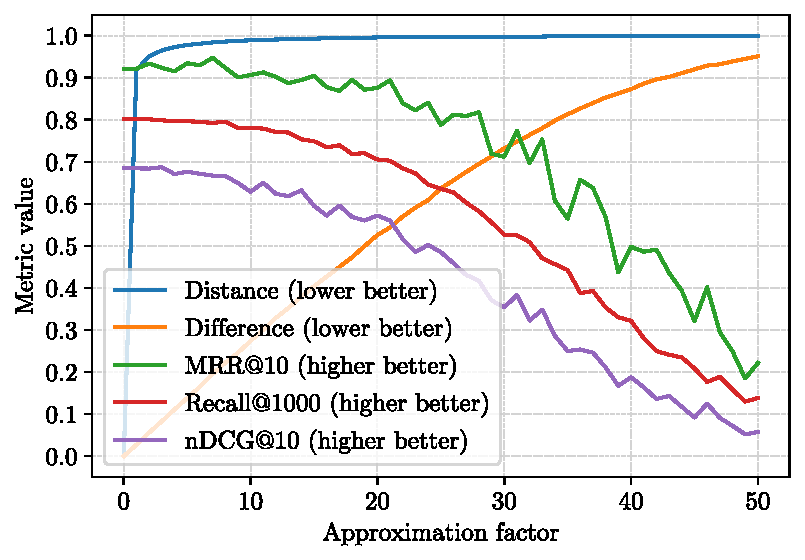
\includegraphics[width=1.0\textwidth]{knn-search-0-50} % chktex 8
	\caption{Search accuracy for $\beta \in \{ 0.0, \ldots, 50.0 \}$}\label{figure:knn-search-coarse}
\end{figure}

		\begin{figure}[h]
	\centering
	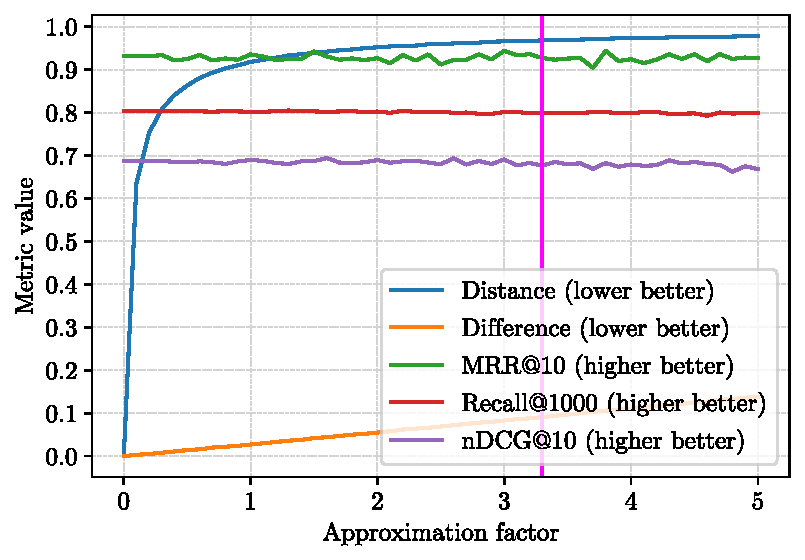
\includegraphics[width=1.0\textwidth]{knn-search-0-5}  % chktex 8
	\caption[Search accuracy for $\beta \in \{ 0.0, \ldots, 5.0 \}$]{
		Search accuracy for $\beta \in \{ 0.0, \ldots, 5.0 \}$.
		{\color{magenta}Highlighted} is $\beta = \sqrt{\max N}$ for $\max N \approx 11$ being the longest vector in the dataset.
	}\label{figure:knn-search-fine}
\end{figure}


	\section{Security against attacks}
